\documentclass[assd_tp3_main.tex]{subfiles}

\begin{document}

\section{Modulador delta}

El segundo conversor anal\'ogico/digital que se implement\'o fue un modulador delta. El mismo hace uso del principio de que, al muestrear una se\~nal a una frecuencia mucho mayor a la de Nyquist (oversampling), el valor de la misma no se altera significativamente entre muestra y muestra. Por lo tanto, codificando la diferencia entre una muestra y la siguiente, en lugar del valor de la muestra en s\'i, se puede ganar SQNR sin necesidad de incrementar el n\'umero de bits del ADC. El diagrama de bloques b\'asico de este conversor se observa en la figura \ref{fig:delta-bloques}.

\begin{figure}[htb]
	\centering
	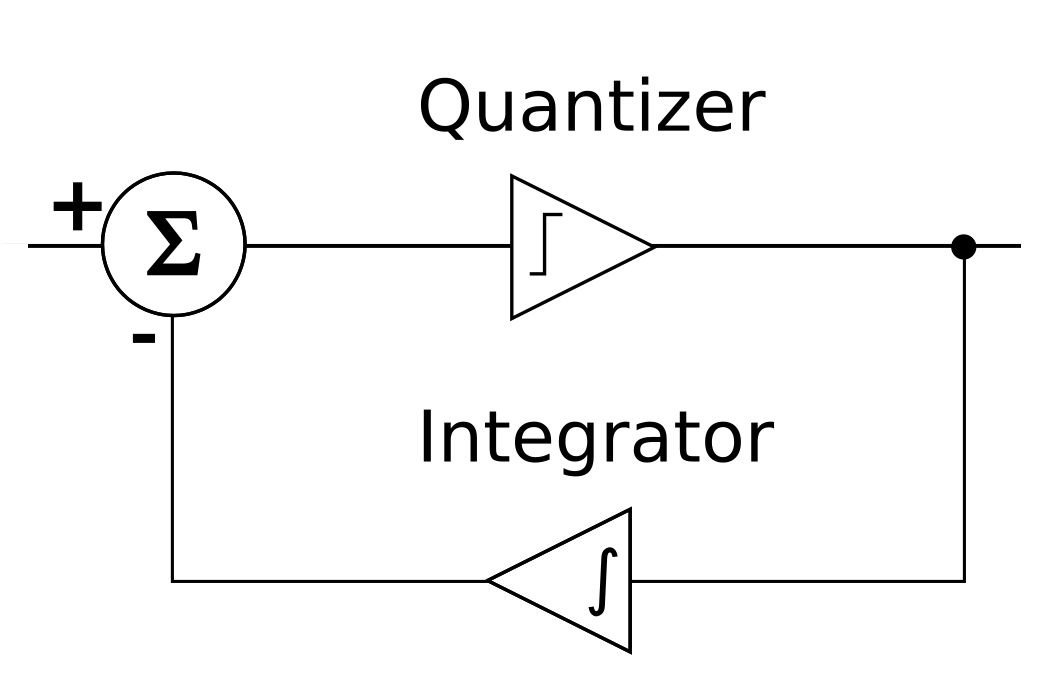
\includegraphics[width=0.6 \textwidth]
	{imagenes/ej3/delta-bloques.png}
	\caption{Diagrama de bloques del modulador delta}
	\label{fig:delta-bloques}
\end{figure}

\end{document}